\documentclass[12pt, letterpaper]{article}

\usepackage[utf8]{inputenc}
\usepackage[spanish, es-tabla]{babel}
\usepackage[margin=2.5cm]{geometry}
\usepackage{graphicx}
\usepackage{float}
\usepackage{hyperref}
\usepackage[numbers,sort&compress]{natbib}
\usepackage{booktabs}
\usepackage{xcolor}
\usepackage{listings}
\graphicspath{{images/}}
\bibliographystyle{ieeetr}

\lstdefinestyle{code}{
    basicstyle=\ttfamily\footnotesize,
    breaklines=true,
    frame=single,
    numbers=left,
    numberstyle=\tiny,
    tabsize=2,
    showstringspaces=false
}
\lstset{style=code}

\begin{document}

\begin{titlepage}
    \centering
    {\bfseries\LARGE Universidad Tecnológica Metropolitana} \\
    \vspace{0.3cm}
    {\large Facultad de Ingeniería / Ingeniería Civil en Electrónica} \\
    \vspace{0.1cm}
    {\large Departamento de Electricidad} \\

    \vspace{1.4cm}
    
\includegraphics[width=0.2\textwidth]{logo_utem.png} \\
    \vspace{1.4cm}

    {\scshape\Large Informe de Laboratorio N°3 y N°4} \\
    \vspace{0.5cm}
    {\bfseries\huge Sistema de visión artificial con Raspberry Pi y ESP32-CAM} \\

    \vfill

    \begin{flushleft}
    \textbf{Asignatura:} Microcontroladores ELEB8092 \\
    \textbf{Profesor:} Dr. Exequiel Álvarez Olate \\
    \textbf{Experiencias:} Vigilancia IoT distribuida y preparación de Raspberry Pi 4
    \end{flushleft}

    \vspace{0.8cm}

    \begin{flushright}
    \textbf{Integrantes:} \\
    Sebastian Espinosa \\
    Axel Valdes \\
    \vspace{0.5cm}
    \textbf{Fecha:} 3 de julio de 2026
    \end{flushright}
\end{titlepage}

\tableofcontents
\newpage

\section{Introducción}

Los laboratorios 3 y 4 tienen un eje común: usar la Raspberry Pi 4 como plataforma de visión artificial y delegar o concentrar tareas de captura según el hardware disponible. En el Laboratorio 3 se implementó una arquitectura distribuida donde una ESP32-CAM transmite video por Wi-Fi y la Raspberry realiza la inferencia. En el Laboratorio 4 se verificó la preparación de la Raspberry como nodo local de visión, incluyendo cámara conectada, OpenCV, YOLOv8 y OCR para patentes.

Para evitar repetir procedimientos equivalentes, este informe integra ambas experiencias en un solo flujo: primero se describe la plataforma común, luego la transmisión IoT con ESP32-CAM y finalmente la prueba ANPR/ALPR solicitada en el Laboratorio 4.

\section{Objetivos}

\begin{itemize}
    \item Configurar la ESP32-CAM AI-Thinker como nodo de captura MJPEG sobre HTTP.
    \item Preparar la Raspberry Pi 4 para recibir video, procesar imágenes y ejecutar inferencia local.
    \item Implementar detección de personas/vehículos con YOLOv8 Nano en formato ONNX.
    \item Implementar el conteo de aforo por línea virtual solicitado como reto del Laboratorio 3.
    \item Validar un flujo de reconocimiento de patentes para el Laboratorio 4 y generar evidencia fotográfica.
\end{itemize}

\section{Marco teórico resumido}

El sistema se basa en una separación de responsabilidades. La ESP32-CAM trabaja como nodo de borde encargado de capturar y transmitir imágenes; la Raspberry Pi 4 actúa como servidor de niebla o nodo de procesamiento. Esta división es necesaria porque la ESP32-CAM no cuenta con recursos suficientes para ejecutar modelos de detección como YOLOv8 en tiempo real.

El video se transmite como MJPEG sobre HTTP, protocolo simple en el que cada frame viaja como una imagen JPEG independiente. OpenCV puede abrir este stream como si fuera una cámara local. Para la inferencia se usó YOLOv8 Nano exportado a ONNX, ejecutado mediante OpenCV DNN, evitando el uso directo de PyTorch debido a incompatibilidades observadas en la Raspberry.

Para el reconocimiento de patentes se evaluó EasyOCR, pero durante la prueba real presentó fallos de \textit{illegal instruction} asociados a PyTorch. Por esta razón se utilizó Tesseract 5.5.0 como ruta OCR operativa, aplicando recorte de la zona de patente, escala de grises, binarización y normalización del texto.

\section{Materiales y software}

\begin{table}[H]
    \centering
    \caption{Elementos utilizados.}
    \begin{tabular}{p{0.36\textwidth} p{0.48\textwidth}}
    \toprule
    \textbf{Elemento} & \textbf{Uso} \\
    \midrule
    Raspberry Pi 4 & Servidor de procesamiento e inferencia. \\
    ESP32-CAM AI-Thinker & Captura y transmisión MJPEG del Laboratorio 3. \\
    Webcam USB Logitech C170 & Cámara local usada para las pruebas del Laboratorio 4. \\
    Fuente externa 5 V & Alimentación estable para la ESP32-CAM. \\
    Arduino CLI y core ESP32 & Compilación y carga del firmware. \\
    Python 3.13, OpenCV, NumPy & Captura, procesamiento y visualización. \\
    YOLOv8n ONNX & Detección de personas y vehículos. \\
    Tesseract 5.5.0 & OCR funcional para patentes. \\
    \bottomrule
    \end{tabular}
\end{table}

\section{Desarrollo}

\subsection{Arquitectura general}

La Figura \ref{fig:arquitectura} resume la arquitectura implementada. La ESP32-CAM transmite frames JPEG por Wi-Fi hacia la Raspberry Pi, donde se ejecuta el pipeline de visión artificial. Para la parte local del Laboratorio 4, la Raspberry también puede capturar directamente desde una cámara USB mediante \texttt{cv2.VideoCapture(0)}.

\begin{figure}[H]
    \centering
    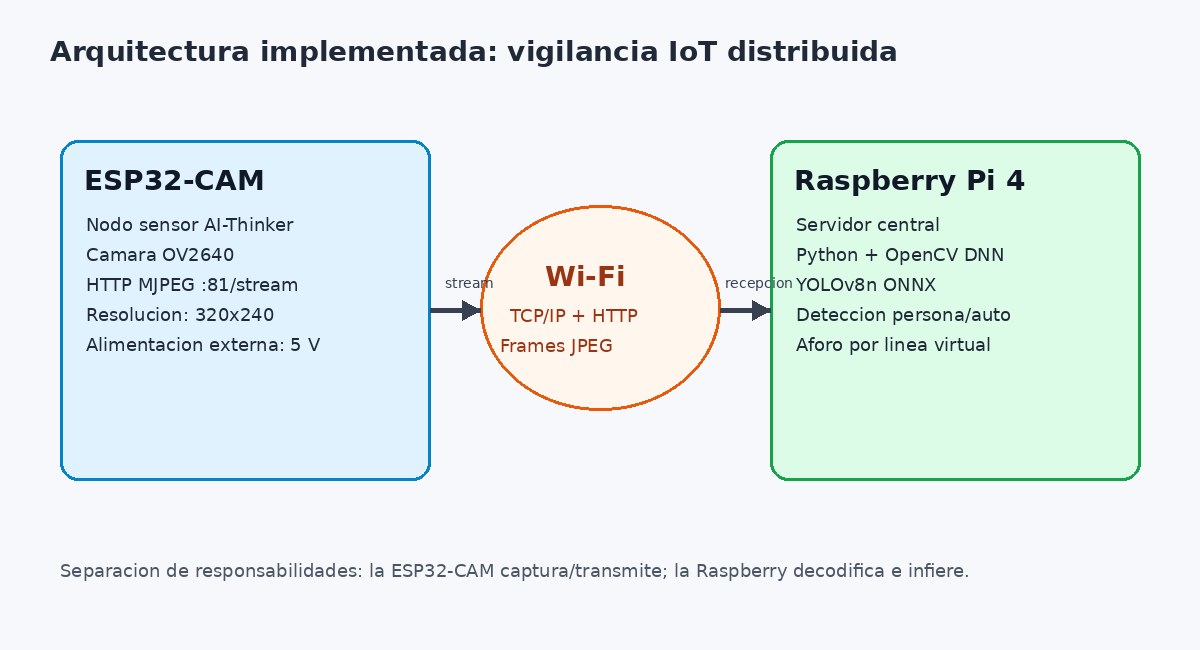
\includegraphics[width=0.92\textwidth]{arquitectura_iot.png}
    \caption{Arquitectura general del sistema de visión artificial.}
    \label{fig:arquitectura}
\end{figure}

\subsection{ESP32-CAM y transmisión MJPEG}

El firmware de la ESP32-CAM inicializa el sensor OV2640, configura salida JPEG y expone dos rutas HTTP: \texttt{/capture} para capturas individuales y \texttt{:81/stream} para video MJPEG continuo. Para mejorar estabilidad y FPS se redujo la resolución a QVGA (320x240), se ajustó la compresión JPEG y se desactivó el ahorro de energía Wi-Fi.

\begin{lstlisting}[language=C++, caption={Configuración aplicada en la ESP32-CAM.}]
config.frame_size = FRAMESIZE_QVGA;
config.jpeg_quality = 16;
config.fb_count = 3;
config.fb_location = CAMERA_FB_IN_PSRAM;

WiFi.mode(WIFI_STA);
WiFi.setSleep(false);
\end{lstlisting}

\subsection{Procesamiento en Raspberry Pi}

La Raspberry recibe el stream desde \texttt{http://172.20.10.12:81/stream}. Para evitar latencia acumulada se implementó lectura en un hilo separado: siempre se procesa el frame más reciente. Además, YOLO se ejecuta cada cuatro frames con \texttt{--infer-every 4}, lo que mejora la fluidez de visualización en CPU.

\subsection{Conteo de aforo}

Para el reto del Laboratorio 3 se dibujó una línea virtual horizontal y se calcularon centroides de las personas detectadas. Cuando un centroide cruza la línea, se actualiza el contador de aforo. La Figura \ref{fig:aforo} muestra una captura real desde la ESP32-CAM con la línea de conteo.

\begin{figure}[H]
    \centering
    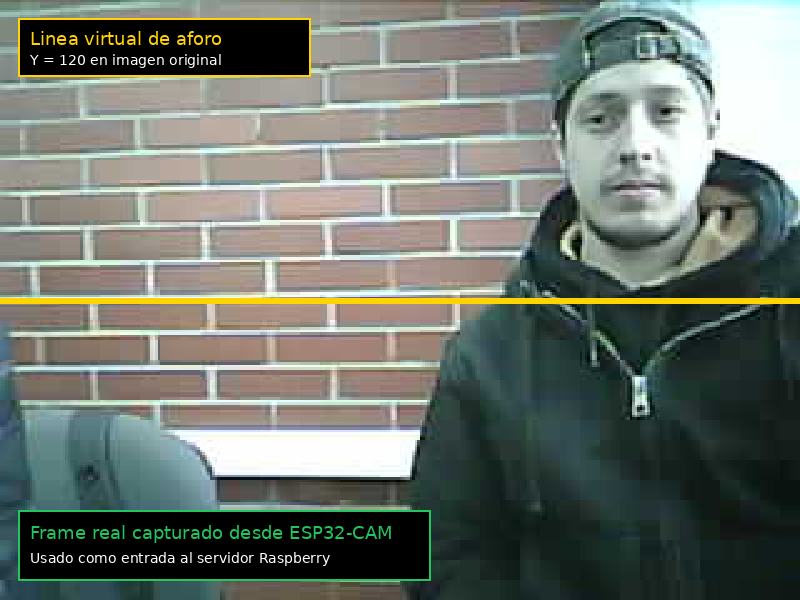
\includegraphics[width=0.72\textwidth]{captura_anotada_aforo.png}
    \caption{Captura real desde ESP32-CAM con línea virtual de aforo.}
    \label{fig:aforo}
\end{figure}

\subsection{Preparación de Raspberry Pi para el Laboratorio 4}

La guía del Laboratorio 4 pide comprobar sistema operativo de 64 bits, entorno virtual, cámara y librerías de visión artificial. En esta Raspberry se verificó OpenCV, Ultralytics, EasyOCR y Tesseract. La cámara CSI/NoIR indicada por la guía no fue detectada por \texttt{rpicam}, pero sí se detectó y probó una webcam USB Logitech C170 en \texttt{/dev/video0}. La captura local funcionó a 640x480.

\begin{lstlisting}[language=bash, caption={Verificación resumida del entorno.}]
Version de Python: 3.13.5
Version de OpenCV: 5.0.0
Ultralytics (YOLOv8): OK
EasyOCR: OK
Tesseract: 5.5.0
Camara funcional. Resolucion del frame: 640 x 480
\end{lstlisting}

\subsection{Reconocimiento de patentes}

Para la prueba ANPR/ALPR se mostró una patente desde un teléfono frente a la cámara. El texto visible fue \texttt{BB-BB-10}. El programa recortó la zona de la patente, aplicó binarización y ejecutó Tesseract. La lectura normalizada fue \texttt{BBBB10}, incluida en la lista de patentes autorizadas. La Figura \ref{fig:anpr} muestra la evidencia final.

\begin{figure}[H]
    \centering
    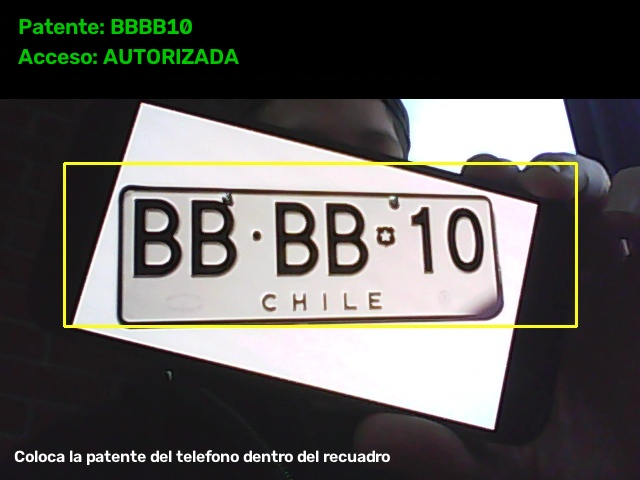
\includegraphics[width=0.72\textwidth]{lab4/anpr_camara_real_resultado.jpg}
    \caption{Reconocimiento de patente con acceso autorizado.}
    \label{fig:anpr}
\end{figure}

\section{Resultados y análisis}

\begin{table}[H]
    \centering
    \caption{Resultados principales.}
    \begin{tabular}{p{0.42\textwidth} p{0.42\textwidth}}
    \toprule
    \textbf{Parámetro} & \textbf{Resultado} \\
    \midrule
    Resolución ESP32-CAM & 320x240 pixeles \\
    IP usada por ESP32-CAM & 172.20.10.12 \\
    Stream & \texttt{http://172.20.10.12:81/stream} \\
    Modelo de detección & YOLOv8n ONNX \\
    Frecuencia de inferencia & 1 inferencia cada 4 frames \\
    FPS observado en prueba & 2.67 FPS de visualización \\
    OCR operativo & Tesseract 5.5.0 \\
    Patente leída & \texttt{BBBB10} \\
    Resultado de acceso & Autorizado \\
    Estado alimentación Raspberry & \texttt{throttled=0x0} \\
    \bottomrule
    \end{tabular}
\end{table}

El rendimiento quedó limitado principalmente por CPU y por la transmisión MJPEG en Wi-Fi. La alimentación externa de 5 V para la ESP32-CAM mejoró estabilidad, evitando reinicios o cortes de stream durante las pruebas. En el caso del OCR, Tesseract resultó más estable que EasyOCR en esta instalación porque no depende de inferencia PyTorch pesada.

\subsection{Cumplimiento de las guías}

\begin{table}[H]
    \centering
    \caption{Comparación con los puntos solicitados.}
    \begin{tabular}{p{0.36\textwidth} p{0.12\textwidth} p{0.36\textwidth}}
    \toprule
    \textbf{Punto solicitado} & \textbf{Estado} & \textbf{Evidencia} \\
    \midrule
    ESP32-CAM programada y transmitiendo por Wi-Fi & Cumplido & Firmware, stream MJPEG y configuración HTTP. \\
    Servidor Raspberry que consume el stream & Cumplido & Script \texttt{rasberryesp32.py} con OpenCV. \\
    Detección con YOLOv8 & Cumplido & Modelo YOLOv8n exportado a ONNX. \\
    Reto Lab 3 & Cumplido & Se implementó el Reto B: conteo de aforo por línea virtual. \\
    Entorno Python bajo PEP 668 & Cumplido & Uso de entorno virtual y dependencias aisladas. \\
    Verificación de cámara en Raspberry & Cumplido con ajuste & No se detectó cámara CSI/NoIR; se usó webcam USB funcional. \\
    Reconocimiento de patentes & Cumplido & Lectura \texttt{BBBB10} y decisión de acceso autorizado. \\
    Alerta o salida de acceso & Cumplido & Señal visual en pantalla: acceso autorizado/no autorizado. \\
    Repositorio de código & Parcial & Se entrega código limpio y \texttt{requirements.txt}; falta subirlo a GitHub si el docente lo exige. \\
    Video demostrativo & Parcial & La demostración fue en vivo; se incluye evidencia fotográfica en el informe. \\
    \bottomrule
    \end{tabular}
\end{table}

\section{Conclusiones}

Se integraron los Laboratorios 3 y 4 en una misma plataforma de visión artificial. El Laboratorio 3 quedó cubierto mediante una ESP32-CAM transmitiendo video a la Raspberry Pi, donde se ejecutó detección con YOLOv8n ONNX y conteo de aforo por línea virtual. El Laboratorio 4 se incorporó como preparación y validación de la Raspberry para visión local, incluyendo cámara USB, entorno Python, OpenCV, OCR y prueba real de patente.

La principal limitación fue el rendimiento de inferencia en CPU. Aun así, el sistema funcionó de forma estable con resolución reducida, lectura asíncrona de frames y OCR basado en Tesseract. La evidencia final demuestra captura, procesamiento, lectura de patente y decisión de acceso autorizado.

\section{Entregables}

\begin{itemize}
    \item Firmware ESP32-CAM: \texttt{esp32\_cam\_stream.ino}.
    \item Servidor Raspberry: \texttt{rasberryesp32.py}.
    \item Scripts Lab 4: pruebas de entorno, captura local, detección,
    ANPR por consola y visor web.
    \item Dependencias Python: \texttt{requirements.txt}.
    \item Modelo: \texttt{yolov8n.onnx}.
    \item Evidencia fotográfica incorporada en este informe.
\end{itemize}

\newpage
\addcontentsline{toc}{section}{Referencias}
\nocite{*}
\bibliography{referencias}

\end{document}
